\documentclass[10pt]{article}

\usepackage{amsmath}
\usepackage{caption}
\usepackage{hyperref}
\usepackage{indentfirst}
\usepackage{subfig}
\usepackage{wrapfig}

\usepackage{fec,homework}

\begin{document}
	\title{Warm Starting Series of Mixed-Integer Linear Programs: \\
		Theory, Implementation, and Application}
	\author{A Dissertation Proposal by Sean Kelley $^a$ \\
		$^a$ Department of Industrial and Systems Engineering, Lehigh University}
	\date{April 18, 2022}
	\maketitle
	
	\bigskip
	
	\begin{abstract}
		Several well known classes of mixed-integer programs (MIP's) rely on solving series of mixed-integer linear programs (MILP's) where each instance differs only by objective coefficients or constraint bounds. Upon solving one MILP instance, attributes of its Branch-and-Cut tree can be reused to generate valid inequalities that tighten the underlying root linear programming (LP) relaxation for unsolved instances in the series. This approach could significantly improve how MILP's in such a series are warm-started today, but does not currently exist. This dissertation proposes the following deliverables to address that gap: publish a new warm-starting methodology with this approach, implement the methodology in open-source, and publish an application of the methodology to a sufficiently structured and common industrial application. This dissertation will yield emperical proof of how to more effectively warm start MILP's in a series and serve as a blueprint for improving solver performance for several classes of MIP's.
	\end{abstract}
	
	\section{Introduction} \label{s:intro}
	
	\subsection{Motivation} \label{ss:motivation}
	Mixed-Intger Programming (MIP) has a deeply studied theory and has been adopted in many successful industrial applications, such as production scheduling, vehicle routing, and facility location. Much of this theory and many of these applications are focused on the case in which a single Mixed-Integer Linear Programming (MILP) instance is solved. Driven by demand for applications to have more precise solutions, this theory has been expanded to enrich the space of solvable MIP instances. Some examples include solving MILP's with many constraints or variables by decomposition methods (electric grid planning and branch and price VRP), MILP's with multiple objectives (multiobjective facility location), MILP's with "real-time" run time restrictions (combinatorial auctions), and Bilevel MILP's (bilevel facility location). With this growth in theory, MIP is more relevant to industry than ever, specifically in the aforementioned applications.
	
	A major bottleneck to implementing applications of more recently developed subclasses of MIP, like those mentioned above, is solving them in a reasonable amount of time. The computational difficultly in the above examples stems from the fact that each relies on solving a series of many MILP instances, formulated as follows:
	\begin{align}
		\begin{split}
			\text{minimize } & {c^k}^T x \\
			\text{subject to } & x \in \mathcal{S}^k
		\end{split} \label{e:milp-k} \tag{MILP-$ k $}
	\end{align}
	where
	\begin{align*}
		\mathcal{S}^{k} = \{x :Ax \geq b^k, \; x_i \in \Zmbb \text{ for all } i \in \mathcal{I} \}
	\end{align*}
	In the above, $ x $ is our variable and $ \mathcal{I} $ is the set of indices of $ x $ that must take on integer values. We assume $ A \in \Rmbb^{m \times n} $, $ b^k \in \Rmbb^m $, and $ c^k \in \Rmbb^n $. For all indices $ k $ and $ l $ in the series, either $ b^k = b^l $ or $ c^k = c^l $.
	
	It is worth noting that solving each instance of \ref{e:milp-k} is already an NP-hard problem. The burden when solving many in a series can be mitigated by "warm starting" each. Specifically, this could include using previously solved problems in the series to calculate what reasonable starting bounds, valid inequalities, or disjunction might be. This allows branch and cut in subsequent solves to bypass primal heuristics and/or initial exploration of the feasible region, and there exists two popular approaches today to accomplish this.
	
	The most recently developed approach trains neural networks to predict primal heuristic and branching decisions made during Branch-and-Bound style algorithms \cite{google}, \cite{l2b}. This enables solvers to more quickly navigate the branch and bound tree for new instances, even remaining effective for less rigidly structured series of instances due to the ability for neural networks to generalize. However, warm-starting with neural networks assumes the availability of the human and computational resources required to accurately train them. Given series of MILPs like \ref{e:milp-k} correspond largely to single problem instances within MIP, training a neural network for each one is intractible.
	
	The traditional approach "reuses the Branch-and-Cut tree" from a previous solve, as is described in \cite{ws}. The primal and dual bounds in a series of MILPs with a fixed coefficient matrix are functions of the objective and constraint bounds. If one can recover those functions from a previously solved instance, they can be reevaluated at the objective and constraint bounds of the new instance to yield its starting bounds. Likewise, when fixing the coefficient matrix, many valid inequalities added during cut generation are functions of the constraint bounds \cite{guz}. These functions can be reevaluated at the constraint bounds of an unsolved instance to generate valid inequalities for it. One more benefit of a fixed coefficient matrix is that Branch-and-Cut for a new instance can be started from the terminal subproblems of a previous instance once their objective and constraint bounds have been updated. Doing so saves the solver from having to branch and bound repeatedly to generate those disjunctive terms. However, when the objective or constraint bounds differ significantly, the reevaluated valid inequalities and bounds can be weak, and Branch-and-Cut may process many subproblems from unneeded disjunctive terms \cite{ws}. Although the above warm starting techniques have little overhead, they can struggle to generalize well for series of MILP instances.
	
	\subsection{Outline} \label{ss:outline}
	The demand for more precise solutions to the applications modeled by MIP's has led to richer, albeit more complex, solution methods, as mentioned in the previous section. For an important subset of these methods, their solves include a series of MILP's with \ref{e:milp-k}'s structure. Given the structure each problem in such series shares with the others, there exists opportunity to warm-start new solves with information from previous ones, significantly improving the performance of the overall solve. However, given the gaps displayed in current warm-starting methodology, an approach that both generalizes well to \ref{e:milp-k} while requiring minimal effort from the practitioner is desired.
	
	This dissertation proposes accomplishing the following to meet this need. First, a new warm starting methodology will be published. In that work, the methodology will show its ability to solve a series of \ref{e:milp-k} more efficiently than current warm starting methods. Second, this methodolgy will be implemented within a COIN-OR package, making this work accessible to the wider research community. Third, in a second publication, the methodology will be applied to a Branch-and-Price formulation of the Capactitated Vehichle Routing Problem with Time Windows, demonstrating its ability to outperform and solve a wider variety of instances than current implementations. Additionally, this publication will be a tutorial to the community of practitioners and researchers as to how they can integrate this warm-starting methodology within MIP algorithms and serve as evidence of this dissertation's effectiveness in practice. The end result will be publications and software that are ready to be built upon by future discrete optimizers.
	
	\section{Disjunctive Cut Warm Start Methodology}
	
	\subsection{Inspiration} \label{ss:inspiration}
	The first deliverable in the dissertation is to develop an improved methodology for warm-starting a series of \ref{e:milp-k}. As shown in section \ref{ss:motivation}, training neural networks for individual MIP instances is cumbersome, so the proposed approach builds off of attributes from Branch-and-Cut trees from previously solved instances in the series. The inspiration is to translate the refined LP relaxation from a solved instance of \ref{e:milp-k} to an unsolved instance while removing all but one node from the queue when Branch-and-Cut begins on the unsolved instance. When compared to traditional warm-starting, this maintains the benefit of starting off with a tightened feasible region while removing the risk that many unneeded subproblems are solved should the objective or constraint bounds change sufficiently. To go deeper into the details of how this works, more notation is needed.
	
	\subsection{Preliminaries} \label{ss:prelims}
	Consider a Branch-and-Cut tree for \ref{e:milp-k}. Node $ t $ in this tree represents a LP subproblem solved during the course of the algorithm. This problem has the following formulation.
	\begin{align}
		\begin{split}
			\text{minimize } & {c^k}^T x \\
			\text{subject to } & x \in \mathcal{P}^{kt}
		\end{split} \label{e:lp-kt} \tag{LP-$ kt $}
	\end{align}
	where
	\begin{align*}
		\mathcal{P}^{kt} &= \{x : A^{tk}x \geq b^{tk}, \; u^{kt} \geq x \geq l^{kt} \} \\
		\mathcal{S}^{kt} &= \{x : x \in \mathcal{P}^{kt}, \; x_i \in \Zmbb \text{ for all } i \in \mathcal{I} \} \\
	\end{align*}
	\begin{align*}
		A^{tk} = \begin{bmatrix} A \\ \Pi^{tk} \end{bmatrix} \text{ and } b^{tk} = \begin{bmatrix} b^k \\ \Pi_0^{tk} \end{bmatrix}
	\end{align*}
	Above, $ u^{kt} $ and $ l^{kt} $ are bounds on $ x $ from branching on ancestor nodes. ($ \Pi^{kt}, \Pi_0^{kt} $) represent constraints added to the LP relaxation from Branch-and-Cut's cut generation subroutine. Another important attribute of this tree is its set of terminal nodes, $ \mathcal{T}^k $, which encodes the final disjunction on the variables.
	
	A main goal of this publication is finding inequalities valid for all nodes in $ \mathcal{T}^k $. For $ \mu^{kt} \in \Rmbb_+^{m}$, $ w^{kt} \in \Rmbb_+^{n}$, $ v^{kt} \in \Rmbb_+^{n} $, and $ I_n $ the $ n $-dimensional identity matrix, the following is a valid inequality for $ \mathcal{P}^{kt} $:
	\begin{align}
		{A^{kt}}^T \mu^{kt} + I_n w^{kt} - I_n v^{kt} \geq {b^{kt}}^T \mu^{kt} + {l^{kt}}^T w^{kt} - {u^{kt}}^T v^{kt} \label{e:lp_kt_valid_inequality} \tag{LP-$ kt $ valid inequality}
	\end{align}
	Let $ \pi \in \Rmbb^n $ and $ \pi_0 \in \Rmbb $ satisfy the following:
	\begin{align}
		\begin{split}
			\pi &\geq {A^{kt}}^T \mu^{kt} + I_n w^{kt} - I_n v^{kt} \\
			\pi_0 & \leq {b^{kt}}^T \mu^{kt} + {l^{kt}}^T w^{kt} - {u^{kt}}^T v^{kt}
		\end{split} \; \text{ for all } t \in \mathcal{T}^k \label{e:k_disjunctive_cut} \tag{$ k $-disjuctive cut}
	\end{align}
	By construction, \ref{e:k_disjunctive_cut} is a \ref{e:lp_kt_valid_inequality} for all $ t \in \mathcal{T}^k $.
	
	Specifically, cuts that refine the underlying LP relaxation for \ref{e:milp-k} near its optimal solution are desired. For $ \bar{x} \Rmbb^n $, an estimate of this solution, such a cut can be found by solving the Cut Generating LP for \ref{e:milp-k}, which is defined as follows:
	\begin{equation} \tag{CGLP-k}
		\begin{alignedat}{2} \label{e:cglp-k} 
			\text{minimize } \; \; \qquad & \pi^T \bar{x} - \pi_0 && \\
			\text{subject to } \qquad \pi & \geq {A^{kt}}^T \mu^{kt} + I_n w^{kt} - I_n v^{kt} && \;  t \in \mathcal{T}^k \\
			\pi_0 & \leq {b^{kt}}^T \mu^{kt} + {l^{kt}}^T w^{kt} - {u^{kt}}^T v^{kt} && \; t \in \mathcal{T} \\
			1 & = \sum_{t \in \mathcal{T}^k} \big( \sum_{j=1}^{m^t} \mu_j^{kt} + \sum_{i=1}^{n} w_i^{kt} + \sum_{i=1}^{n} v_i^{kt} \big) && \\
			& \mu^{kt} \in \Rmbb_+^{m^t}, \; w^{kt} \in \Rmbb_+^n \; v^{kt} \in \Rmbb_+^n && t \in \mathcal{T}^k
		\end{alignedat}
	\end{equation}
	The added constraint from \ref{e:k_disjunctive_cut} to \ref{e:cglp-k} is for normalization to ensure the optimal solution is finite. In order to scale this LP to many disjunctive terms, a more performant variant \cite{aleks} will be implemented and used for testing. Going forward, \ref{e:cglp-k}($\bar{x}'$) means to solve \ref{e:cglp-k} with $ \bar{x} = \bar{x}' $. The above explains how to find \ref{e:k_disjunctive_cut}s for a solved \ref{e:milp-k}. The following shows a similar procedure can be used to find $ l $-disjunctive cuts for an unsolved MILP-$ l $.
	
	In the case that $ b^k = b^l $ and the same disjunction is applied, the cuts generated in each node $ t $ remain valid for $ \mathcal{S}^{lt} $. Therefore, one can solve \ref{e:cglp-k}($ \bar{x}^l $) to find $ l $-disjunctive cuts.
	
	In the case that $ c^k = c^l $ and the same disjunction is applied, each \ref{e:lp-kt} can be transformed to generate LP-$ lt $ such that it is a relaxation of $ \mathcal{S}^{lt} $. Begin by replacing $ b^k $ with $ b^l  $. Then overload $ \Pi_0^{kt} $ to map $ b^l $ such that $ (\Pi^{kt}, \Pi_0^{kt}(b^l)) $ become valid inequalities for the integer points in LP-$ lt $. For this publication, Gomory Mixed-Integer Cuts (GMICs) will be the only cuts used beyond those generated from the CGLP. See \cite{guz} for map details. Doing this yields the following constraints within $ \mathcal{P}^{lt} $
	\begin{align*}
		A^{lt} = \begin{bmatrix} A \\ \Pi^{kt} \end{bmatrix} \text{ and } b^{lt} = \begin{bmatrix} b^l \\ \Pi_0^{kt}(b^l) \end{bmatrix}
	\end{align*}
	Each of these terms can be substituted in \ref{e:cglp-k} to yield \ref{e:cglp-l}, which, given, $ \bar{x} $, an estimate solution to MILP-$ l $, is formulated as follows:
	\begin{equation} \tag{CGLP-l}
		\begin{alignedat}{2} \label{e:cglp-l} 
			\text{minimize } \; \; \qquad & \pi^T \bar{x} - \pi_0 && \\
			\text{subject to } \qquad \pi & \geq {A^{lt}}^T \mu^{lt} + I_n w^{lt} - I_n v^{lt} && \;  t \in \mathcal{T}^k \\
			\pi_0 & \leq {b^{lt}}^T \mu^{lt} + {l^{lt}}^T w^{lt} - {u^{lt}}^T v^{lt} && \; t \in \mathcal{T}^k \\
			1 & = \sum_{t \in \mathcal{T}^k} \big( \sum_{j=1}^{m^t} \mu_j^{lt} + \sum_{i=1}^{n} w_i^{lt} + \sum_{i=1}^{n} v_i^{lt} \big) && \\
			& \mu^{lt} \in \Rmbb_+^{l^t}, \; w^{lt} \in \Rmbb_+^n \; v^{lt} \in \Rmbb_+^n && t \in \mathcal{T}^k
		\end{alignedat}
	\end{equation}
	Analygous to \ref{e:cglp-k}, let \ref{e:cglp-l}($ \bar{x}' $) represent solving \ref{e:cglp-l} with $ \bar{x} = \bar{x}' $.

	Warm starting MILP-$ l $ with disjunctive cuts means the following: Wtih a (partially) solved \ref{e:milp-k}, construct and run \ref{e:cglp-k}($\bar{x}'$) if $ b^k = b^l $ or \ref{e:cglp-l}($\bar{x}'$) if $ b^k \neq b^l $ for all $\bar{x}'$ solution estimates of MILP-$ l $. Add the resulting cut(s) to the root relaxation of MILP-$ l $ and start Branch-and-Cut with the tightened root relaxation. Add further disjuctive cuts to the subtree rooted at a node $ t $ by solving \ref{e:cglp-k}($ \bar{x}^{lt} $) or \ref{e:cglp-l}($ \bar{x}^{lt} $) as appropriate where $ \bar{x}^{lt} $ is the solution to LP-$ lt $.
	
	\subsection{Numerical Experiments} \label{ss:numerical_experiments}
	There are three sets of experiments this publication will run, exploring each of the three possible cases for warm-starting MILP-$ l $ with disjunctive cuts: $ c^l = c^k $ and $ b^l = b^k $, $ c^l = c^k $ but $ b^l \neq b^k $, and $ c^l \neq c^k $ but $ b^l = b^k $. The procedure and deliverable for each experiment is as follows.
	
	\subsubsection{Restarting \ref{e:milp-k}} \label{sss:restarting_milp_k}
	
	In the case that $ c^l = c^k $ and $ b^l = b^k $, MILP-$ l $ is the same as \ref{e:milp-k}. This scenario can explore if it is possible to partially solve \ref{e:milp-k} then warm-start with disjunctive cuts and solve to optimality MILP-$ l $ in less time than solving \ref{e:milp-k} to optimality alone. The first experiment of this publication will test to see which classes of MILP instances, if any, this happens. The deliverable will be a list of which MILP classes can be solved more efficiently in this manner.
	
	Identifying such classes comes down to collecting and displaying a set of metrics while solving \ref{e:milp-k} and its disjunctive-cut warm-started peer, as initial runs will likely not yeild expected results and will lead to further refinements. To test if changing parameters affects the benefit of warm-starting, the following graphs are broken out by how many nodes are processed before restarting in the warm-start case, and whether or not variable bounds and the constraint matrix of \ref{e:cglp-k} accumulate as the solve progresses. When variable bounds are cumulative while solving \ref{e:cglp-k} at node $ t $, for all nodes $ t' \in \mathcal{T}^k $, $ l^{kt} = $ max$ \{ l^{kt}, l^{kt'} \} $ and $ u^{kt} = $ min$ \{u^{kt}, u^{kt'} \} $. No updates to variable bounds are made in the case that they are fixed. When constraint bounds are cumulative while solving \ref{e:cglp-k} at node $ t $, for all nodes $ t' \in \mathcal{T}^k $, $ \Pi^{t'k} = \Pi^{tk} $. Like the variable bounds, no updates to constraint matrices are made in the case that they are fixed. With the exception of figure \ref{f:cglp_usage}, the graphs display a ratio of the warm and cold started cases. Thus, a positive number represents an improvement from warm-starting.
	
	How often a node $ t $ fails to find a cut from \ref{e:cglp-k} that refines \ref{e:lp-kt} is the first metric tracked and is displayed in figure \ref{f:cglp_usage}. On average, 80\% to 90\% of nodes processed do not use the cut generated from \ref{e:cglp-k}. Since \ref{e:cglp-k} is constructed from 4 and 16 node disjunctions, this is an expected result, as the warm-started Branch and Bound tree does not need to be very deep before \ref{e:cglp-k} no longer generates cuts for a node $ t $ that refine \ref{e:lp-kt}. This does, however, show that disjunctive cuts are used with a significant frequency, thus their effect may be felt by the performance of warm-started solves.
	
	\begin{figure}[h]
		\centering
		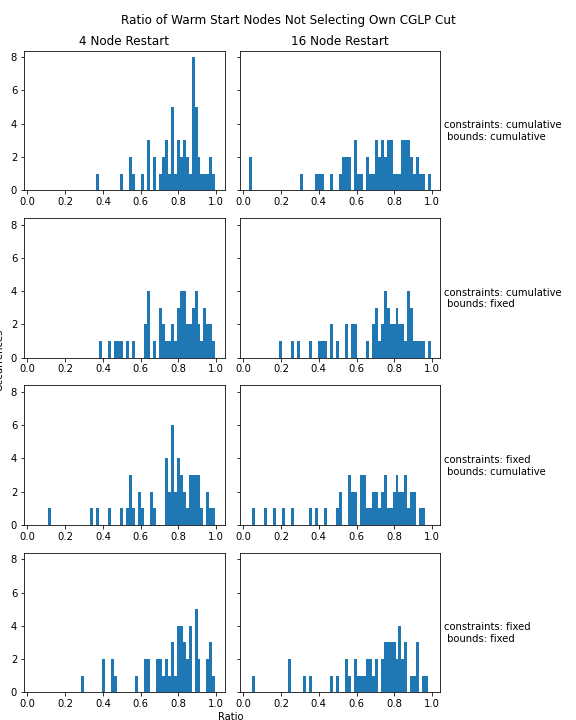
\includegraphics[width=0.5\textwidth]{Ratio of Warm Start Nodes Not Selecting Own CGLP Cut.png}
		\caption{Ratio of nodes processed when warm-starting \ref{e:milp-k} that ignore the cut generated from \ref{e:cglp-k}}
		\label{f:cglp_usage}
	\end{figure} 
	
	The first place to check for this performance improvement is in how much the initial dual bound improves after solving LP-$ k0 $, the root node relaxation for both the warm and cold started cases. Figure \ref{f:initial_dual_gap} illustrates this by plotting the ratio of the dual gaps after solving the root relaxations. The figure shows the extra cut added to LP-$ k0 $ does improve the dual bound by a couple percent on average, meaning that it is possible for the warm-started instances to see better overall solve performance.
	
	\begin{figure}[h]
		\centering
		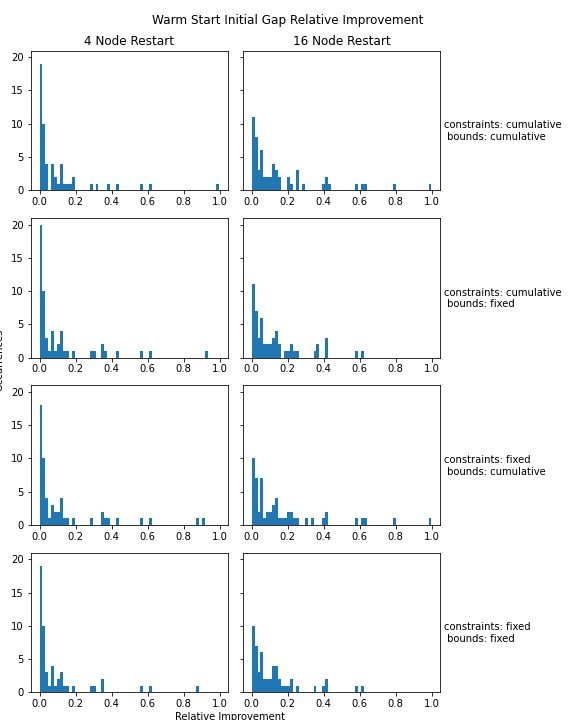
\includegraphics[width=0.5\textwidth]{Warm Start Initial Gap Relative Improvement.png}
		\caption{Ratio of dual gaps after solving the root relaxation for warm and cold started \ref{e:milp-k} instances}
		\label{f:initial_dual_gap}
	\end{figure} 

	The first place to check if the overall solve is improved is the number of nodes both the warm and cold started \ref{e:milp-k}'s had to process. The ratio of those two values is graphed in figure \ref{f:warm_start_nodes}. This set of graphs reveals that in most cases adding cuts from \ref{e:cglp-k} leads to processing more nodes, which is the opposite of what is expected with tighter \ref{e:lp-kt}'s. To prove that warm-starting \ref{e:milp-k} is a viable approach to its solve, this dissertation will need to show that warm-starting reduces the number of nodes processed, which means it would then be plausible for warm-starting to reduce the run time compared to a cold start.
	
	\begin{figure}[h]
		\centering
		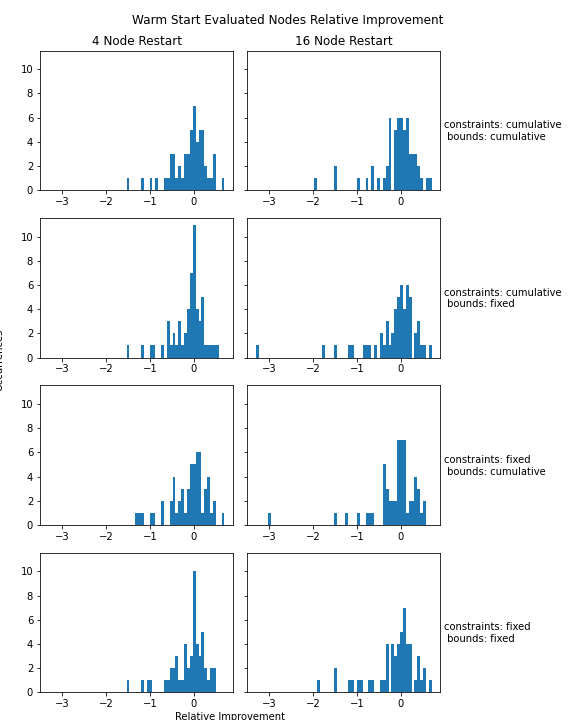
\includegraphics[width=0.5\textwidth]{Warm Start Evaluated Nodes Relative Improvement.png}
		\caption{Ratio of number of nodes processed for warm and cold started \ref{e:milp-k} instances}
		\label{f:warm_start_nodes}
	\end{figure}
	
	\subsubsection{Warm Starting MILP-\boldmath\texorpdfstring{$ l $}{l} When \boldmath\texorpdfstring{$ c^l \neq c^k $}{cl not equal ck} or \boldmath\texorpdfstring{$ b^l \neq b^k$}{bl not equal bk}} \label{sss:warm_starting_milp_l}
	
	Once shown that it is plausible to warm-start \ref{e:milp-k} more effectively than cold-starting, this dissertation will test the ability for disjuctive cuts from \ref{e:milp-k} to warm-start MILP-$ l $. Similar to the data displayed in Section \ref{sss:restarting_milp_k}, both experiments in this section will be checked for how the root dual bound and total number of processed nodes changes between warm and cold starts.
	
	Stepping up in complexity, the case that $ c^l \neq c^k $ but $ b^l = b^k $ will be tested next. This experiment will determine when warm-starting MILP-$ l $ with disjunctive cuts leads to a faster solve than the traditional warm-start approach and no warm-starting at all. In this experiment, since the feasible regions of \ref{e:milp-k} and MILP-$ l $ are the same, the initial solution estimates used for warm-starting could include all feasible solutions found to \ref{e:milp-k}. Additionally, the solution to the LP relaxation of \ref{e:milp-k} could be used. For determining when warm-starting MILP-$ l $ with disjunctive cuts has the best performance, various degrees of change between $ c^l $ and $ c^k $ will be tested as will different classes of \ref{e:milp-k}. The deliverable is a range of classes of \ref{e:milp-k} and angles between $ c^l $ and $ c^k $ such that warm-starting MILP-$ l $ with disjunctive cuts leads to the most efficient solve.
	
	Lastly, the case that $ c^l = c^k $ but $ b^l \neq b^k $ will be tested. This experiment will warm-start MILP-$ l $ when $ b^k \neq b^l $ as proposed in the previous section. This experiment will proceed in the same way as the previous experiment and yield the same format of result.
	
	\subsection{Implications Moving Forward} \label{ss:implications}
	In the near term, further work improving the algorithms that generate and select disjunctive cutting planes is needed. It is a reasonable expectation that warm-starting \ref{e:milp-k} with its own disjunctive cuts as in section \ref{sss:restarting_milp_k} should see a reduction in number of nodes processed when solving. There could currently be a few reasons why this issue is occurring, and the current priority is to explore each to find potential improvements.
	
	The first issue is that numerical errors could be hampering the accuracy of the cuts. In rare cases, the underlying optimization software that solves \ref{e:cglp-k} returns the wrong optimal solution. This could be happening more than is expected, which would reduce the quality of the cuts added to each \ref{e:lp-kt}. To fix this, tests on smaller models that can be debugged need to be run to confirm \ref{e:cglp-k} is implemented correctly.
	
	Another issue that comes to mind is that \ref{e:cglp-k} is not large enough to be effective. When the disjunction is only a few terms, \ref{e:cglp-k} is limited in the depth of cuts it can create as the disjunction is very similar to the root LP relaxation. Currently, it is hard to solve much larger instances of \ref{e:cglp-k} than tested in section \ref{sss:restarting_milp_k}, but \cite{aleks} gives multiple ideas for how this computation can be improved. With those ideas implemented, future experiments can create better disjunctive cuts, possibly yielding more promising results.
	
	One last issue to explore would be generating more than one cut from \ref{e:cglp-k} in each cut generation iteration. When \ref{e:cglp-k} is solved, it is relatively cheap computationally to find many nearby solutions, which are also valid inequalities for \ref{e:milp-k}. Augmenting the disjunctive cut generation subroutine to return many valid inequalities that could potentially be used to tighten \ref{e:lp-kt} may help improve the overall solve performance by reducing the space needing searched for solutions.
	
	Once the above changes are made and the three experiments are complete, there should ranges for classes of MILP's and degree of similarity between \ref{e:milp-k} and MILP-$ l $ that suggest which approach should be used to warm-start the latter given the former has already been partially solved. This information can be used to further improve the performance increase due to warm-starting classes of MIP reliant on solving series of \ref{e:milp-k}. 
	
	\section{Implementing Disjunctive Cut Warm Starts} \label{s:implementing}
	
	\subsection{Motivation} \label{ss:implementation_motivation}
	Before disjunctive warm-starts can improve the performance of classes of MIP reliant on solving series of \ref{e:milp-k}, the code for disjunctive warm-starting must be open-sourced. Once open-sourced, the code will be available to the research community, enabling them to make those improvements. Further, another advantage of open-sourcing is that the code can integrate with a popular open-source solver (like CBC, SYMPHONY, or SCIP). The intention in this dissertation in doing the latter is to give legitimacy to experimental results found in the first publication. To implement disjunctive warm-starts in open-source, the following will need to be done.
	
	\subsection{Cut Generation Routine} \label{ss:cut_generation}
	First, a cut generation routine, which accepts a list of terminal subproblems to a solved \ref{e:milp-k} and a list of solution estimates to an unsolved MILP-$ l $, must solve the appropriate CGLP and return the corresponding deepest cuts. For this to work, this dissertation will include adding a tree that tracks the generated subproblems for the augmented solver's Branch-and-Cut class if it does not already exist. Additionally, if there are subproblems that are optimized in a presolved space, then a subroutine will be developed to map preprocessed variables and constraint bounds back to the original problem space. With this information, the appropriate CGLP will be formulated and converted to the formulation of \cite{aleks}. Then the found cuts will be returned.
	
	For this to happen, all that remains is implementing the CGLP, and the approach depends on how \ref{e:milp-k} and MILP-$ l $ relate to one another. In the case that $ b^k = b^l $, then, as explained in section \ref{ss:prelims}, \ref{e:cglp-k} can be formulated directly from the Branch-and-Cut class's tree attribute. Another step or two will be required when $ b^k \neq b^l $ to implement \ref{e:cglp-l}. In this case, all cuts added will need to either be removed or translated to remain valid. For the sake of balancing simplicity and effectiveness, only GMIC's will be considered for translation. Therefore, at a minimum, a subroutine to remove cuts generated will be developed. If it is a reasonable effort, attributes will be added to each subproblem tracking which cut types correspond to which rows of \ref{e:lp-kt} and the parameters that generate each GMIC so they can be re-evaluated at $ b^l $. After developing these subroutines and applying them to the Branch-and-Bound class's tree for \ref{e:milp-k}, the tree can build the CGLP in any case considered.
	
	\subsection{Warm Start Class} \label{ss:warm_start_class}
	Beyond a cut generation method, the other piece to implement is a warm-starting class, which has one defining attribute and method each. The attribute of this class is a list of \ref{e:milp-k} represented as Branch-and-Bound objects. The method accepts a MILP-$ l $ and a specification to warm-start with \ref{e:milp-k} such that $ b^k = b^l $ or $ c^k = c^l $. It then calls the new cut generation routine using the Branch-and-Bound object from the nearest sufficient \ref{e:milp-k} and the solution to LP-$ l0 $, the LP relaxation of MILP-$ l $, adding the resulting cut to LP-$ l0 $. (Nearest in this case means most parallel objectives if $ b^k = b^l $ or smallest eucidian distance between constraint bounds if $ c^k = c^l $.) The method finishes by running the solve routine on MILP-$ l $'s Branch-and-Bound instance. Optionally, this method could also invoke Branch-and-Bound to include CGLP in its cut generation routine to possibly further improve performance. Lastly, the class instantiates an object with a Branch-and-Bound instance it then solves and places in its attribute's list.
	
	\subsection{Implications Moving Forward} \label{ss:implementation_implications}
	With an open-sourced implementation, the first publication of this dissertation can guide future research efforts as to how classes of MIP's solving series of \ref{e:milp-k} should be warm started.
	
	\section{Applying Disjunctive Cut Warm Starts}
	
	\subsection{Motivation} \label{ss:application_motivation}
	As mentioned earlier, the objective with this dissertation is to advance understanding of how to warm start series of \ref{e:milp-k}'s and ensure its incorporation into future research. The former will be accomplished by the above publication and open-source contribution. The second publication of this disseration will accomplish the latter by providing context on the effectiveness and ease of disjunctive cut warm starting in practice. Specifically, the second publication will solve the Capacitated Vehicle Routing Problem with Time Windows (CVRPRTW) via Branch-and-Price where the pricing problem is solved as a series of \ref{e:milp-k}'s warm started with disjunctive cuts. This dissertation picks this problem and approach for the following reasons.
	
	Branch-and-Price is one of the most commonly applied methods that solves a series of \ref{e:milp-k}, and the CVRPTW is one of the most impactful problems solved with that approach. Thus, showing performance improvements in solving this problem would have immediate impact for how this problem is solved in practice. This kind of accomplishment would generate additional attention for this dissertation's first publication and open-source software contribution, greatly improving the likelihood the research community builds upon those works.
	
	Further, this publication explores warm-starting the CVRPTW with Branch-and-Price because it can be improved along multiple frontiers. Current approaches to the CVRPTW with Branch-and-Price use the pricing problem to generate routes and the master problem to select the optimal subset of routes generated that ensure demand is met \cite{vrp-bap}. In such approaches, route generation is relaxed so Dynamic Programming can solve it, as using MILP is thought to be too inefficient.
	
	This presents two opportunities. First, warm-starting the pricing problem with disjunctive cuts will challenge the notion that Dynamic Programming (DP) is more efficient. The pricing problem is solved many times, increasing the effectiveness of warm-starts, possibly to the extent that solving MILP's is faster than DP's. Second, the DP relaxation of the pricing problem removes the ability for practitioners to add on "side-constraints" that ensure CVRPTW respect real-world restrictions. As \cite{ehsan} shows, side-constraints are a necessary feature of industrial CVRPTW implementations, which is keeping the benefits of Branch-and-Price from being realized at the highest level of impact. Since warm-starting with disjunctive cuts enables solving the full pricing problem efficiently, this publication promises to change that.
	
	Ancillary motivations exist because the CVRPTW is well studied. For one, there exists a rich sample set of instances to test against. As a result, this publication will show how broadly it is effective against current Branch-and-Price implementations, lending further credibility to the results. Further, Branch-and-Price approaches to CVRPTW are well known, allowing the changes in implementation to incorporate disjunctive cut warm-starts to stand out. The result here is an explicit tutorial on how to apply this dissertation's methodology so it can be applied elsewhere.
	
	\subsection{Numerical Experiments} \label{ss:apply_experiments}
	The above section largely spells out what this publication intends to test. The recap is as follows. Both experiments will solve an array of instances of the CVRPTW with Branch-and-Price. The following is how they differ.
	
	In the first experiment, instances will be restricted to those whose pricing problem can be solved with DP. Each instance will have its pricing problem solved as a DP then as a \ref{e:milp-k} warm-started with disjunctive cuts. This will show over what range of instances warm-starting with disjunctive cuts is more efficient than solving a DP.
	
	In the second experiment, instances with challenging pricing problems that cannot be solved with DP will be chosen. This experiment will compare warm-starting the pricing problem to cold starts and heuristic methods to profile how all three approaches differ in terms of solution quality and efficiency. The deliverable is to show under what circumstances pricing problems that cannot be solved with DP's should be warm-started and how impactful is such an approach as compared to cold-starting.
	
	\subsection{Implications of Applying Disjunctive Cut Warm-Starts} \label{ss:application_impllications}
	The implications of applying the first two parts of this dissertation are the motivation, which is mentioned above. To recap, disjunctive cut warm-starts should be applied to Branch-and-Price approaches to the CVRPTW because it is an impactful application in which this dissertation's previous contributions will be effective. Additionally, since Branch-and-Price is well known, this publication will serve as an effective tutorial as to how future publications can apply the earlier works of this dissertation. Collectively, those two results will highlight the utility of this dissertation and prototype future research directions.
		
	\section{Conclusion}\label{s:conclusion}
	In conclusion, this dissertation will develop a new warm-starting methodology, implementation, and application by leveraging disjunctive cuts. It contributes a novel idea to the discrete optimization community with clear directions on how and where to build upon it in the future. Given the breadth of research activity required and that much of the work has and will be done remotely, this dissertation ensures my development into an independent researcher, the main goal of the Ph.D. program. For these reasons, I propose this research plan for my dissertation.
	
	\newpage
	
	\bibliographystyle{plainurl}
	\bibliography{reference}
	
\end{document}